\documentclass{article}
\usepackage{calc}
\usepackage{ifthen}
\usepackage{tikz}
\usepackage[utf8]{inputenc}
\usepackage[T1]{fontenc}
\usepackage{txfonts}
\title{Relatório de Notas de Cálculo A\\Semestre 2016.1}
\author{Melissa Weber Mendonça}
\date{Sábado, 16 de maio de 2016}
\begin{document}
\maketitle
\section*{Distribuição de Notas}
\begin{figure}[ht]
\begin{center}
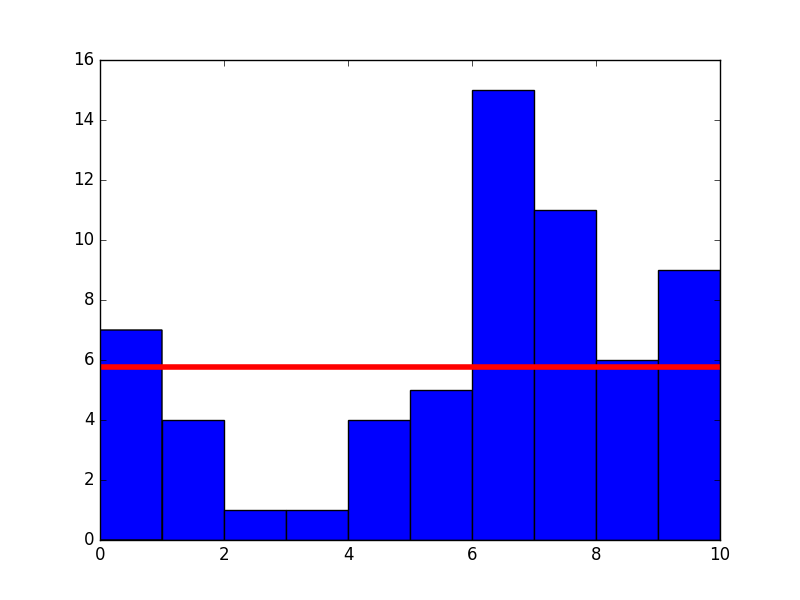
\includegraphics{prova1.png}
\end{center}
\caption{Notas da Prova 1.}
\end{figure}
\begin{figure}[ht]
\begin{center}
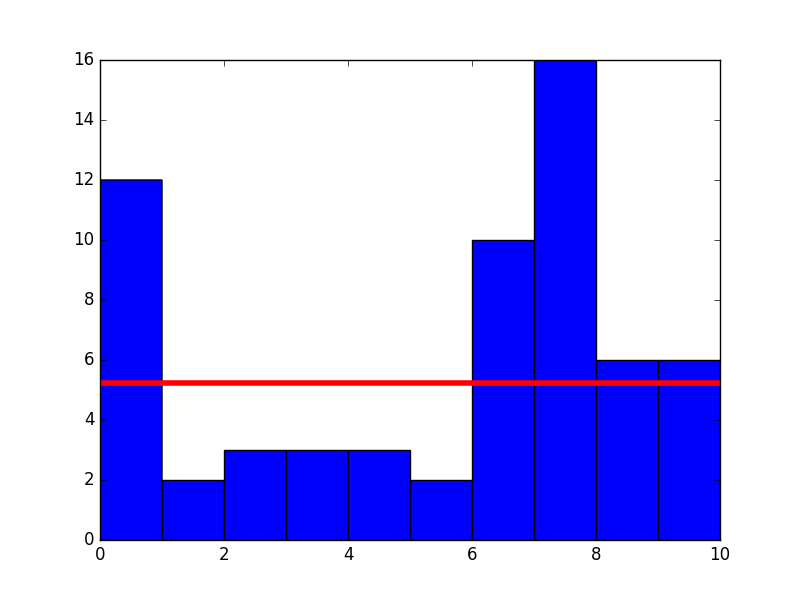
\includegraphics{prova2.png}
\end{center}
\caption{Notas da Prova 2.}
\end{figure}
\begin{figure}[ht]
\begin{center}
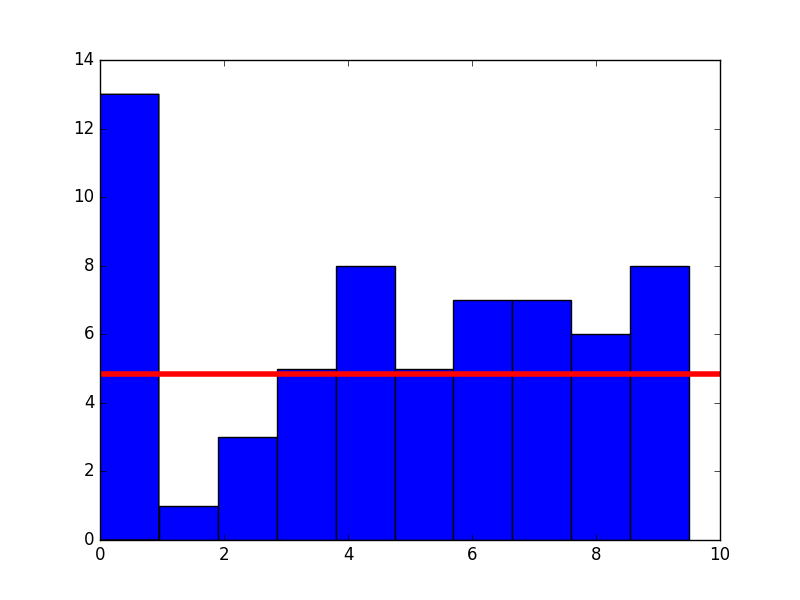
\includegraphics{prova3.png}
\end{center}
\caption{Notas da Prova 3.}
\end{figure}
\end{document}
